\documentclass[a4paper,12pt]{article}

\usepackage{amsmath, amssymb}
\usepackage{gvv}
\usepackage{geometry}
\usepackage{hyperref}
\usepackage{titlesec}
\usepackage{graphicx}
\geometry{margin=1in}

\title{\textbf{7.4.12}}
\author{\textbf{Aditya Mishra — EE25BTECH11005}}
\date{October 12, 2025}

\begin{document}

\maketitle

\section*{Question}
The centres of a set of circles, each of radius \(3\), lie on the circle \(x^2 + y^2 = 25\).  
Find the locus of any point \(\vec{x}\) in the set.

\section*{Solution}

For a circle,
\begin{align}
\vec{u} = -\vec{c}, \quad f = \|\vec{u}\|^2 - r^2
\end{align}
Hence, the general equation is
\begin{align}
\|\vec{x}\|^2 + 2\vec{u}^T\vec{x} + f = 0
\end{align}

For this family,
\begin{align}
\|\vec{u}\| = 5, \quad r = 3, \quad f = 25 - 9 = 16
\end{align}
Thus,
\begin{align}
\|\vec{x}\|^2 + 2\vec{u}^T\vec{x} + 16 \le 0
\end{align}
\begin{align}
2\vec{u}^T\vec{x} \le -\|\vec{x}\|^2 - 16
\end{align}
Since \(\|\vec{u}\| = 5\), by Cauchy-Schwarz inequality:
\begin{align}
-5\|\vec{x}\| \le \vec{u}^T\vec{x} \le 5\|\vec{x}\|
\end{align}

The minimum value of \(2\vec{u}^T\vec{x}\) is \(-10\|\vec{x}\|\).  
Hence, existence requires
\begin{align}
-10\|\vec{x}\| \le -\|\vec{x}\|^2 - 16
\end{align}

\begin{align}
\Rightarrow \|\vec{x}\|^2 - 10\|\vec{x}\| + 16 \le 0
\end{align}

Let \(t = \|\vec{x}\|\). Then
\begin{align}
t^2 - 10t + 16 \le 0
\end{align}
\begin{align}
\Rightarrow (t - 2)(t - 8) \le 0
\end{align}
\begin{align}
\Rightarrow 2 \le t \le 8
\end{align}

\section*{Locus}
\begin{align}
2 \le \|\vec{x}\| \le 8
\quad \Rightarrow \quad
4 \le \vec{x}^T\vec{x} \le 64
\end{align}
\[
\boxed{4 \le x^2 + y^2 \le 64}
\]
\begin{figure}[h!]
    \centering
    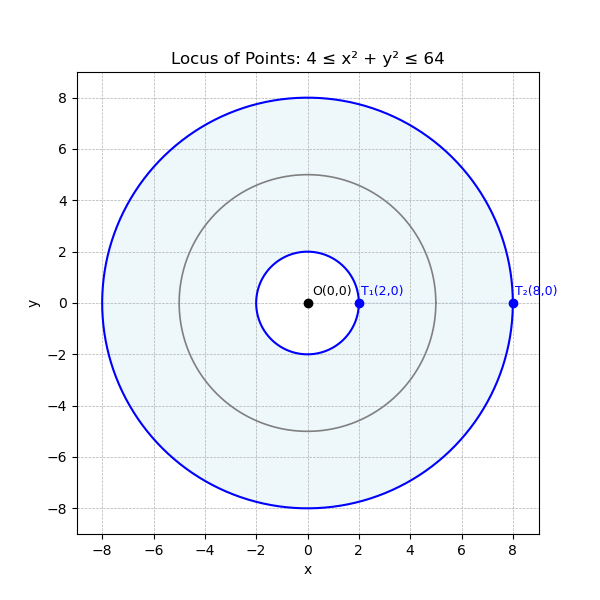
\includegraphics[width=0.7\linewidth]{Figs/Figure_1.png}
    \caption{Locus of points for circles of radius 3 with centers on $x^2 + y^2 = 25$.}
    \label{fig:locus}
\end{figure}

\end{document}

